\section{Data Acquisition}
fNIRS data was collected using two NIRSport2 systems (NIRx Medical Technologies, Berlin, Germany). 
Each NIRSport2 system was equipped with 16 source and 16 detector optodes, and daisy-chained together for a high density 32x32 optode configuration. 
Each neighboring pair of source and detector optode is referred to as a channel, resulting in a total of 103 HbO + 103 HbR channels (plus 16 short distance channels).
The average distance between source and detector optodes was 30 mm, and 7mm for short distance channels, which were placed on a flexible fNIRS head cap (NIRScap) 58 cm in circumference. 
The optodes were arranged in a high density 32x32 montage with one bundle of short distance channels, as shown in Figure \ref{fig:montage}. 
This montage was designed to cover a maximally large area of the brain, given increasing evidence that emotion processing is not localized to specific discrete areas of the brain, rather distributed across the brain \citep{lindquist_brain_2012}. 
The fNIRS cap and optodes were positioned following the 10-20 international coordinate system.
Light was emitted at 760 nm and 850 nm wavelengths, and the sampling rate was approximately 6.105 Hz.

\begin{figure}[H]
    \centering
    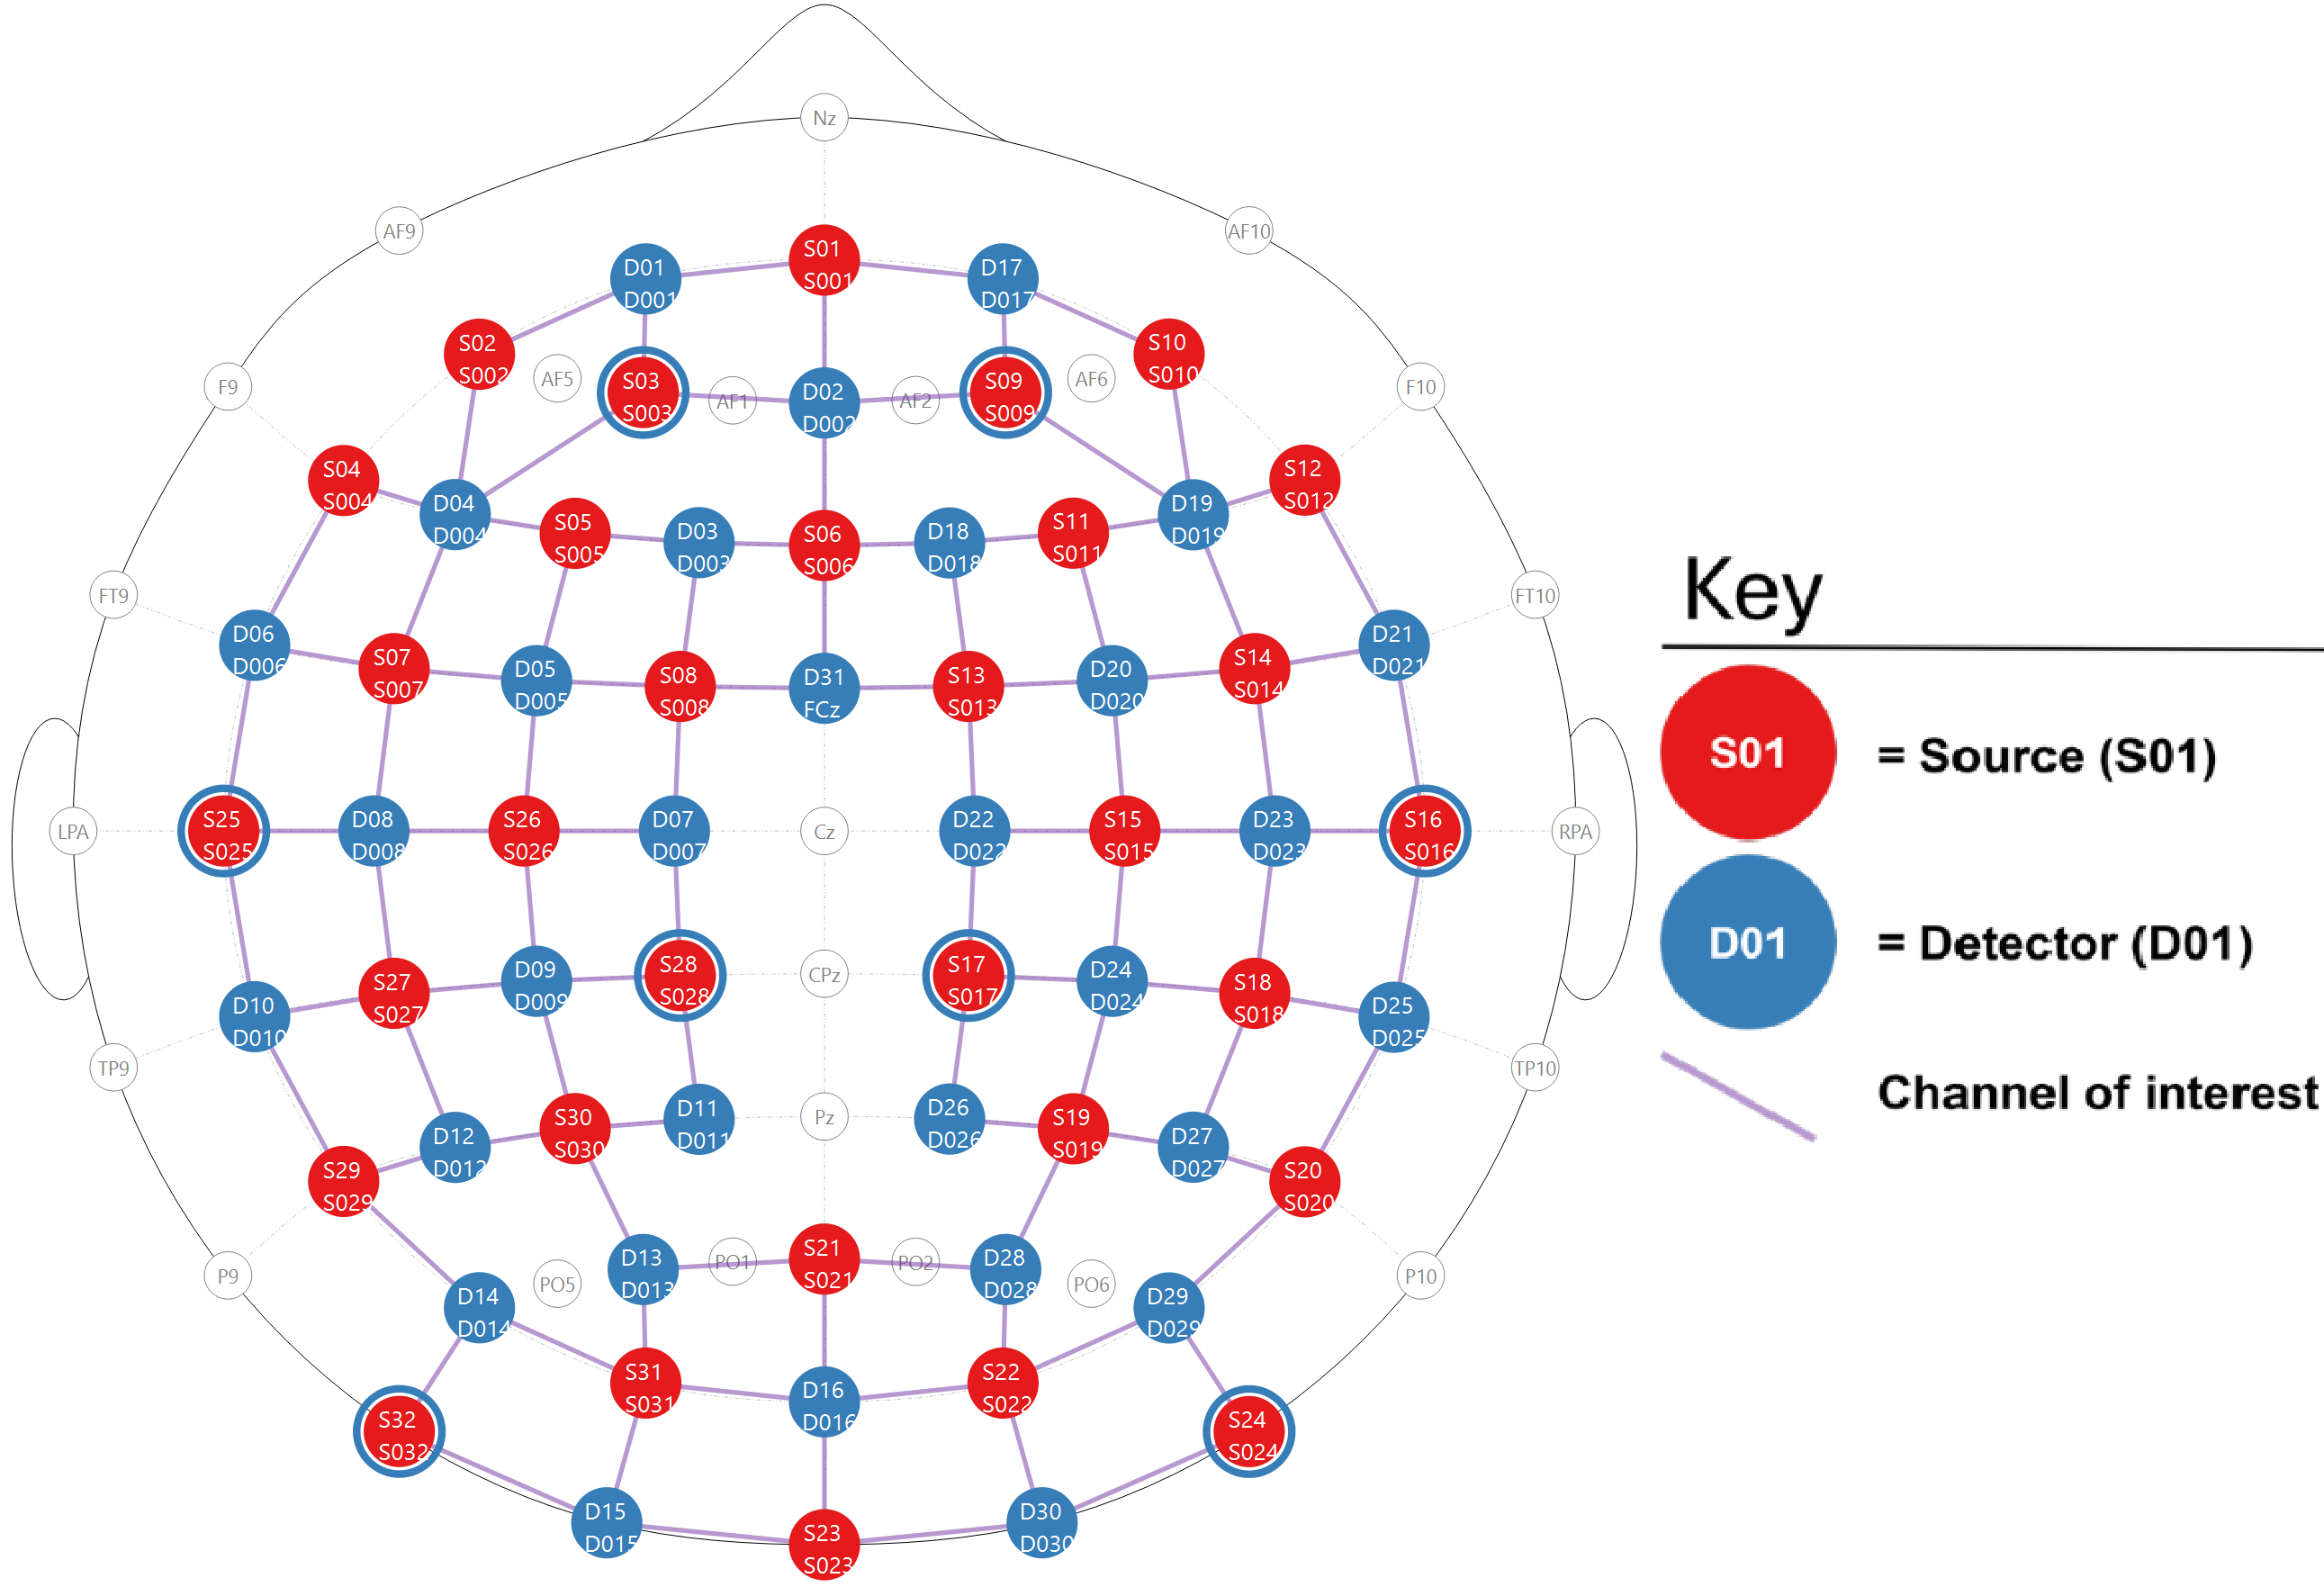
\includegraphics[width=0.6\textwidth]{C:/Users/super/OneDrive - Ontario Tech University/fNIRS_Emotions/plots/figures/Montage.png}
    \caption{2D depiction of the high density 32x32 optode montage, red circles represent sources, blue circles
    represent detectors, purple lines represent channels, and blue rings around sources represent the locations of the 8 short distance detectors. }
    \label{fig:montage}
\end{figure}

\section{Participants}
Participants were recruited from Ontario Tech University's SONA system. 
91 participants completed the study, however 3 were removed due to recording issues, leaving 88 participants.
Signal quality was assessed using the following criteria, similar to \citep{bulgarelli_growth_2025} and \citep{hernandez_nirsplot_2020}: 
Sliding windows of 5 seconds were taken from each channel, and Peak Spectral Power (PSP) and the Scalp Coupling Index (SCI) \citep{pollonini_phoebe_2016} were calculated for each window.
If PSP $>$ 0.1 and SCI $>$ 0.5 for more than 70\% of the windows, the channel was considered to have good signal quality.
If $>$ 70\% of channels were considered to have good signal quality, the participant was included in the analysis.
The minimum SCI threshold was set to 0.5, used in \citep{holmes_opening_2024}, however other studies have used SCI thresholds as low as 0.25\citep{zhou_autistic_2024}. 
After applying these criteria, 53 participants were included in the analysis. 
All participants met the PSP threshold, but only 53/88 met the SCI threshold, as shown in Figure \ref{fig:signal_quality}.
The 53 participants ranged in age from 17 to 51 (M = 21.60, SD = 6.61), and no demographic information was collected. 

\begin{figure}[H]
    \centering
    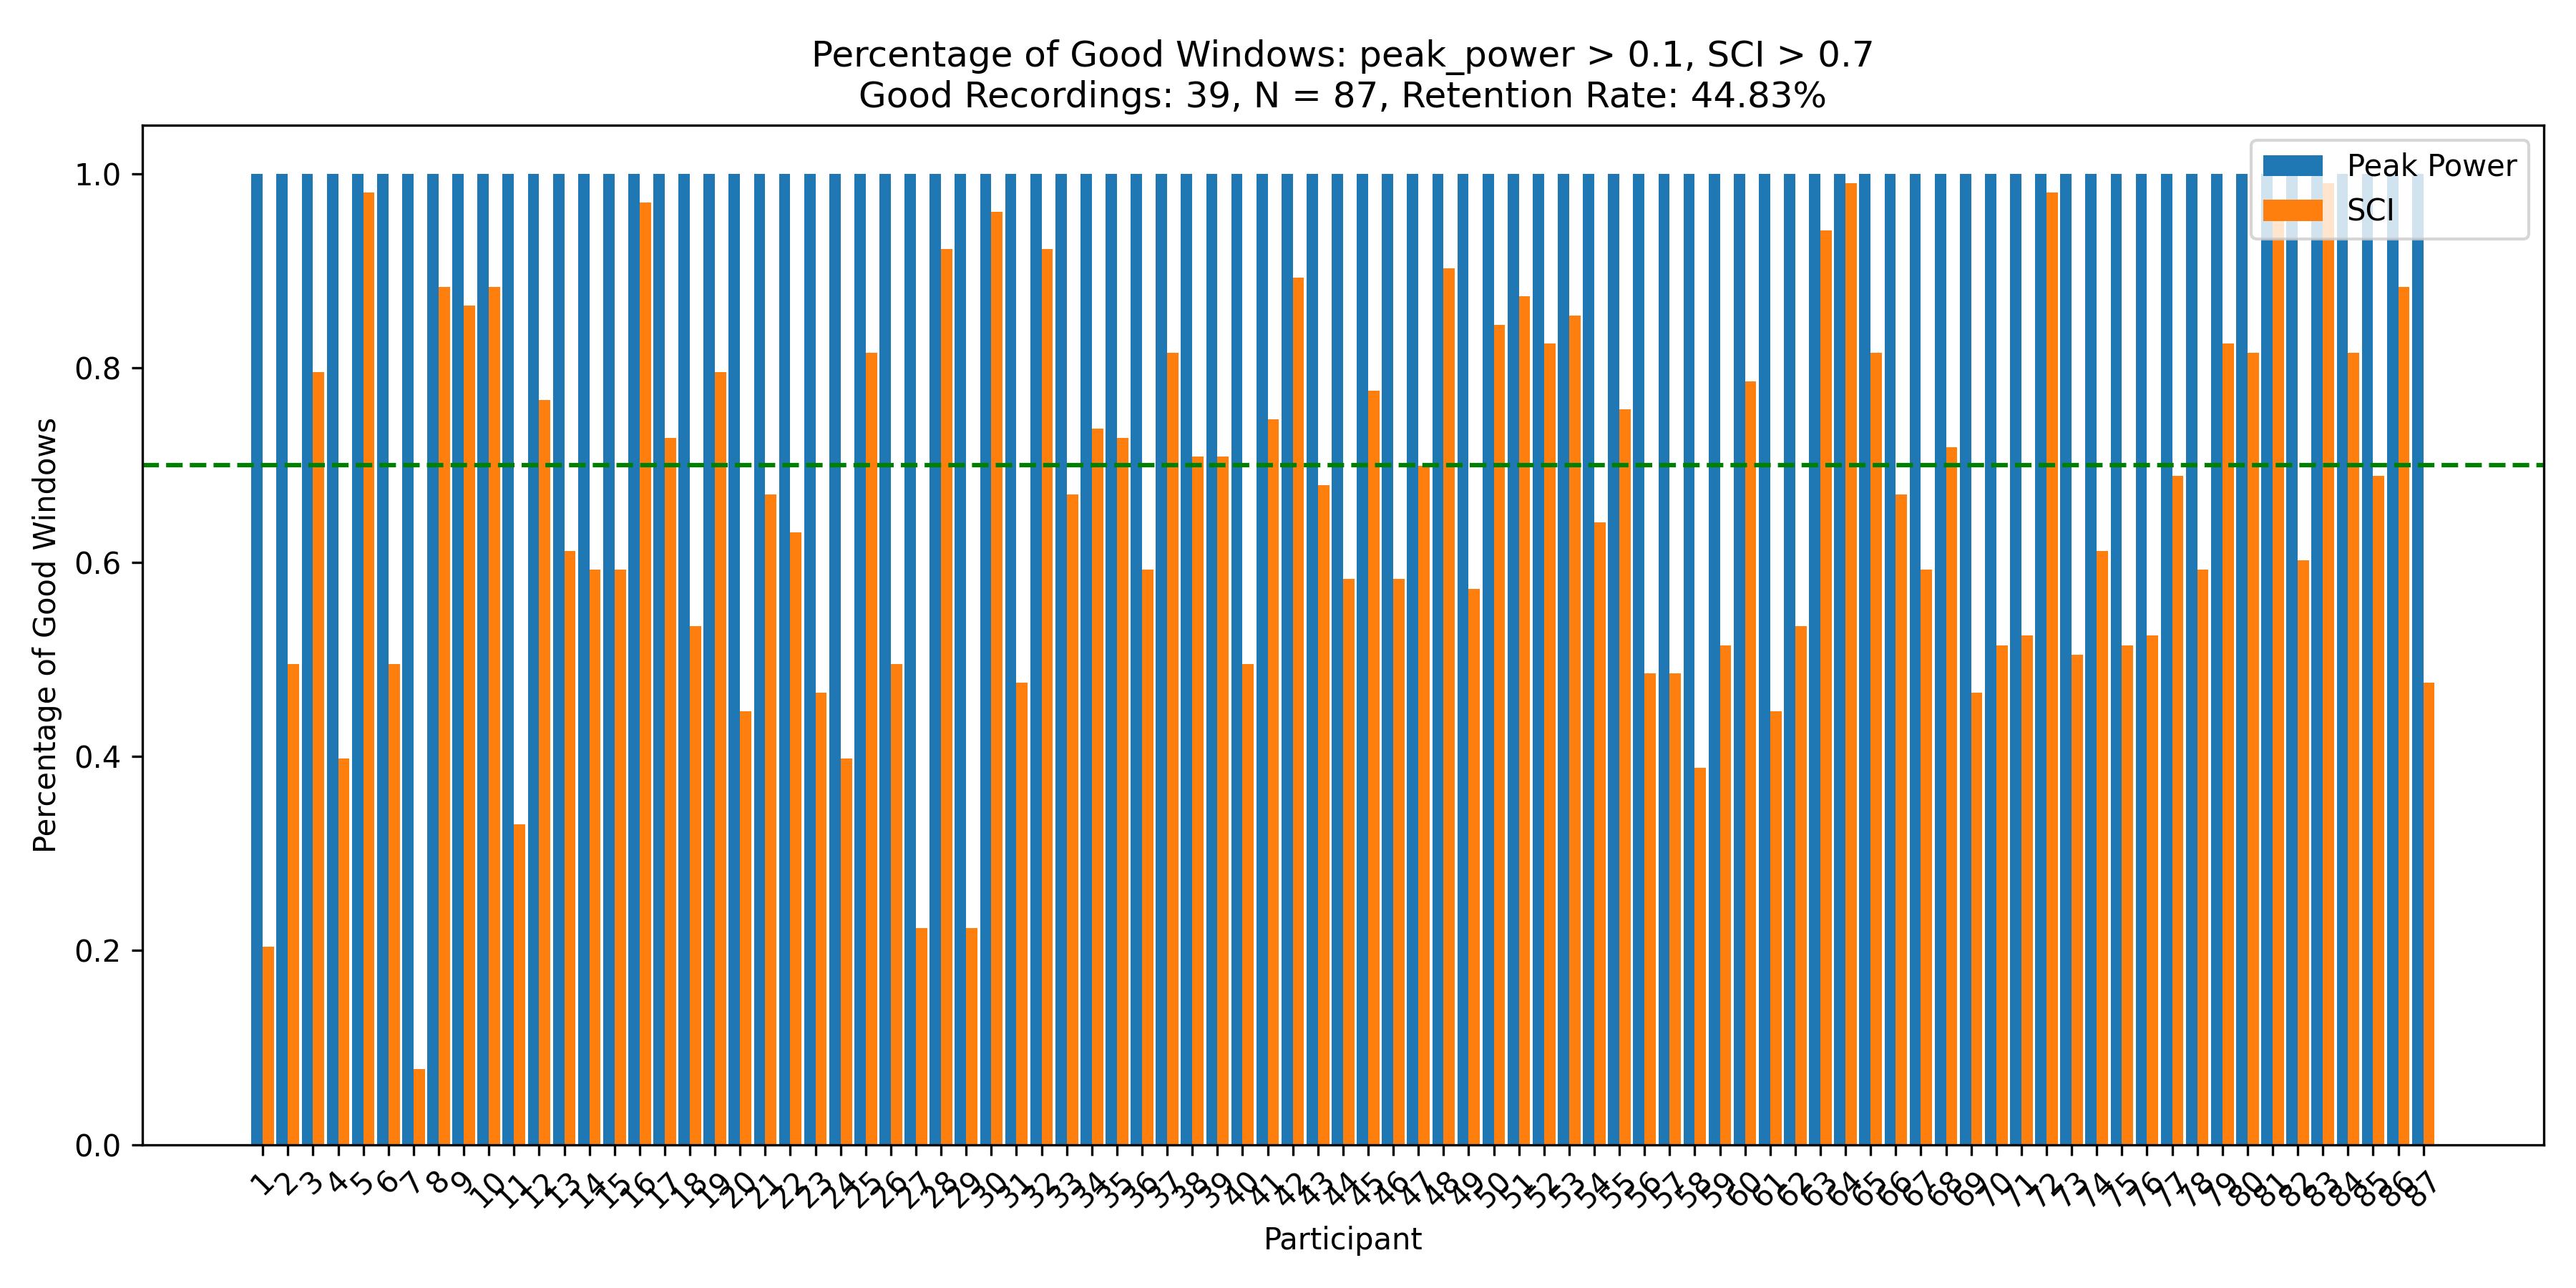
\includegraphics[width=0.9\textwidth]{C:/Users/super/OneDrive - Ontario Tech University/fNIRS_Emotions/plots/signal quality/Percentage of Good Windows.png}
    \caption{Percentage of Channels where SCI $>$ 0.5 for $>$ 70\% of the windows.
    The green dashed line represents the threshold of 70\% of windows that each participant must meet to be included in the analysis.}
    \label{fig:signal_quality}
\end{figure}

\section{Experimental Paradigm}
\subsection{Participant Instructions}
Upon entering the lab, the participant was greeted by the experimenter and asked to read and sign a consent form. 
Their head size was then measured using a tape measure, and the fNIRS cap was fitted to their head as the fNIRS cap was explained to them.
The participant waited patiently while the experimenter(s) checked the signal quality in Aurora fNIRS, the acquisition software for the NIRSport2 system.
The experimenter(s) then attempted to move the participants' hair out of the way of the optodes, to improve signal quality.
The experimenter(s) then explained the task to the participant, and notified them of the camera/microphone in the back of the room. 
No emphasis was given on what to focus on during the task, all the participant was told is that they will be seeing many different types of faces, and that they need to complete the memory task, which is as follows:

\textbf{Memory Task:}
The participant will see blocks of 8 faces, and after each block, there will be a 9th face, and they will need to indicate whether the 9th face was in the previous block of 8 faces.
The participant was instructed to press 'y' on the keyboard if the face was in the previous block, or 'n' if the face was not in the previous block.
This task is visualized in Figure \ref{fig:paradigm}. 

The experimenter(s) then turned the lights off in the room to avoid any interference with the fNIRS cap. 
Then the experimenter(s) started the experiment, and left the room to minimize noise and distractions.
Experimenter(s) then monitored the experiment from outside the room. 
After the experiment was completed (about 35 minutes later), the experimenter(s) entered the room, removed the fNIRS cap, and the participant was given a debriefing letter to read and take home. 
The main purpose of the memory task was to keep the participant engaged and focused on the faces, the memory task was not the main focus of the study, and this was divulged to the participant if they inquired about it after the experiment was completed.

\subsection{Facial Expression Dataset Selection}
Faces were picked from two datasets: the RADIATE dataset \citep{conley_racially_2018} and the UIBVFED dataset \citep{oliver_uibvfed_2020}. 
The RADIATE dataset is a set of 16 emotional expressions by over 100 racially and ethnically diverse real people. 
The UIBVFED dataset is a set of 32 emotional expressions by 20 virtual characters that are also ethnically diverse. 
The faces used in the stimuli presentation were picked carefully with some criteria in mind:
\begin{itemize}
    \item 20 models were selected, 5 males, 5 females from both datasets (RADIATE and UIBVFED). 
    \item The corresponding models from each dataset were matched as closely as possible, in terms of each model's face shape, skin tone, and hair color. 
    \item 7 emotional expressions (anger, disgust, fear, happiness, sadness, surprise, neutral) were selected for each model, that mostly closely align with Ekman's 6 basic emotions + neutral \citep{ekman_are_1992}.
\end{itemize}

The UIBVFED images were cropped to the same size as the RADIATE images, so now a presentation of the stimuli can be created. 

\subsection{Stimuli Presentation}
\begin{figure}[H]
    \centering
    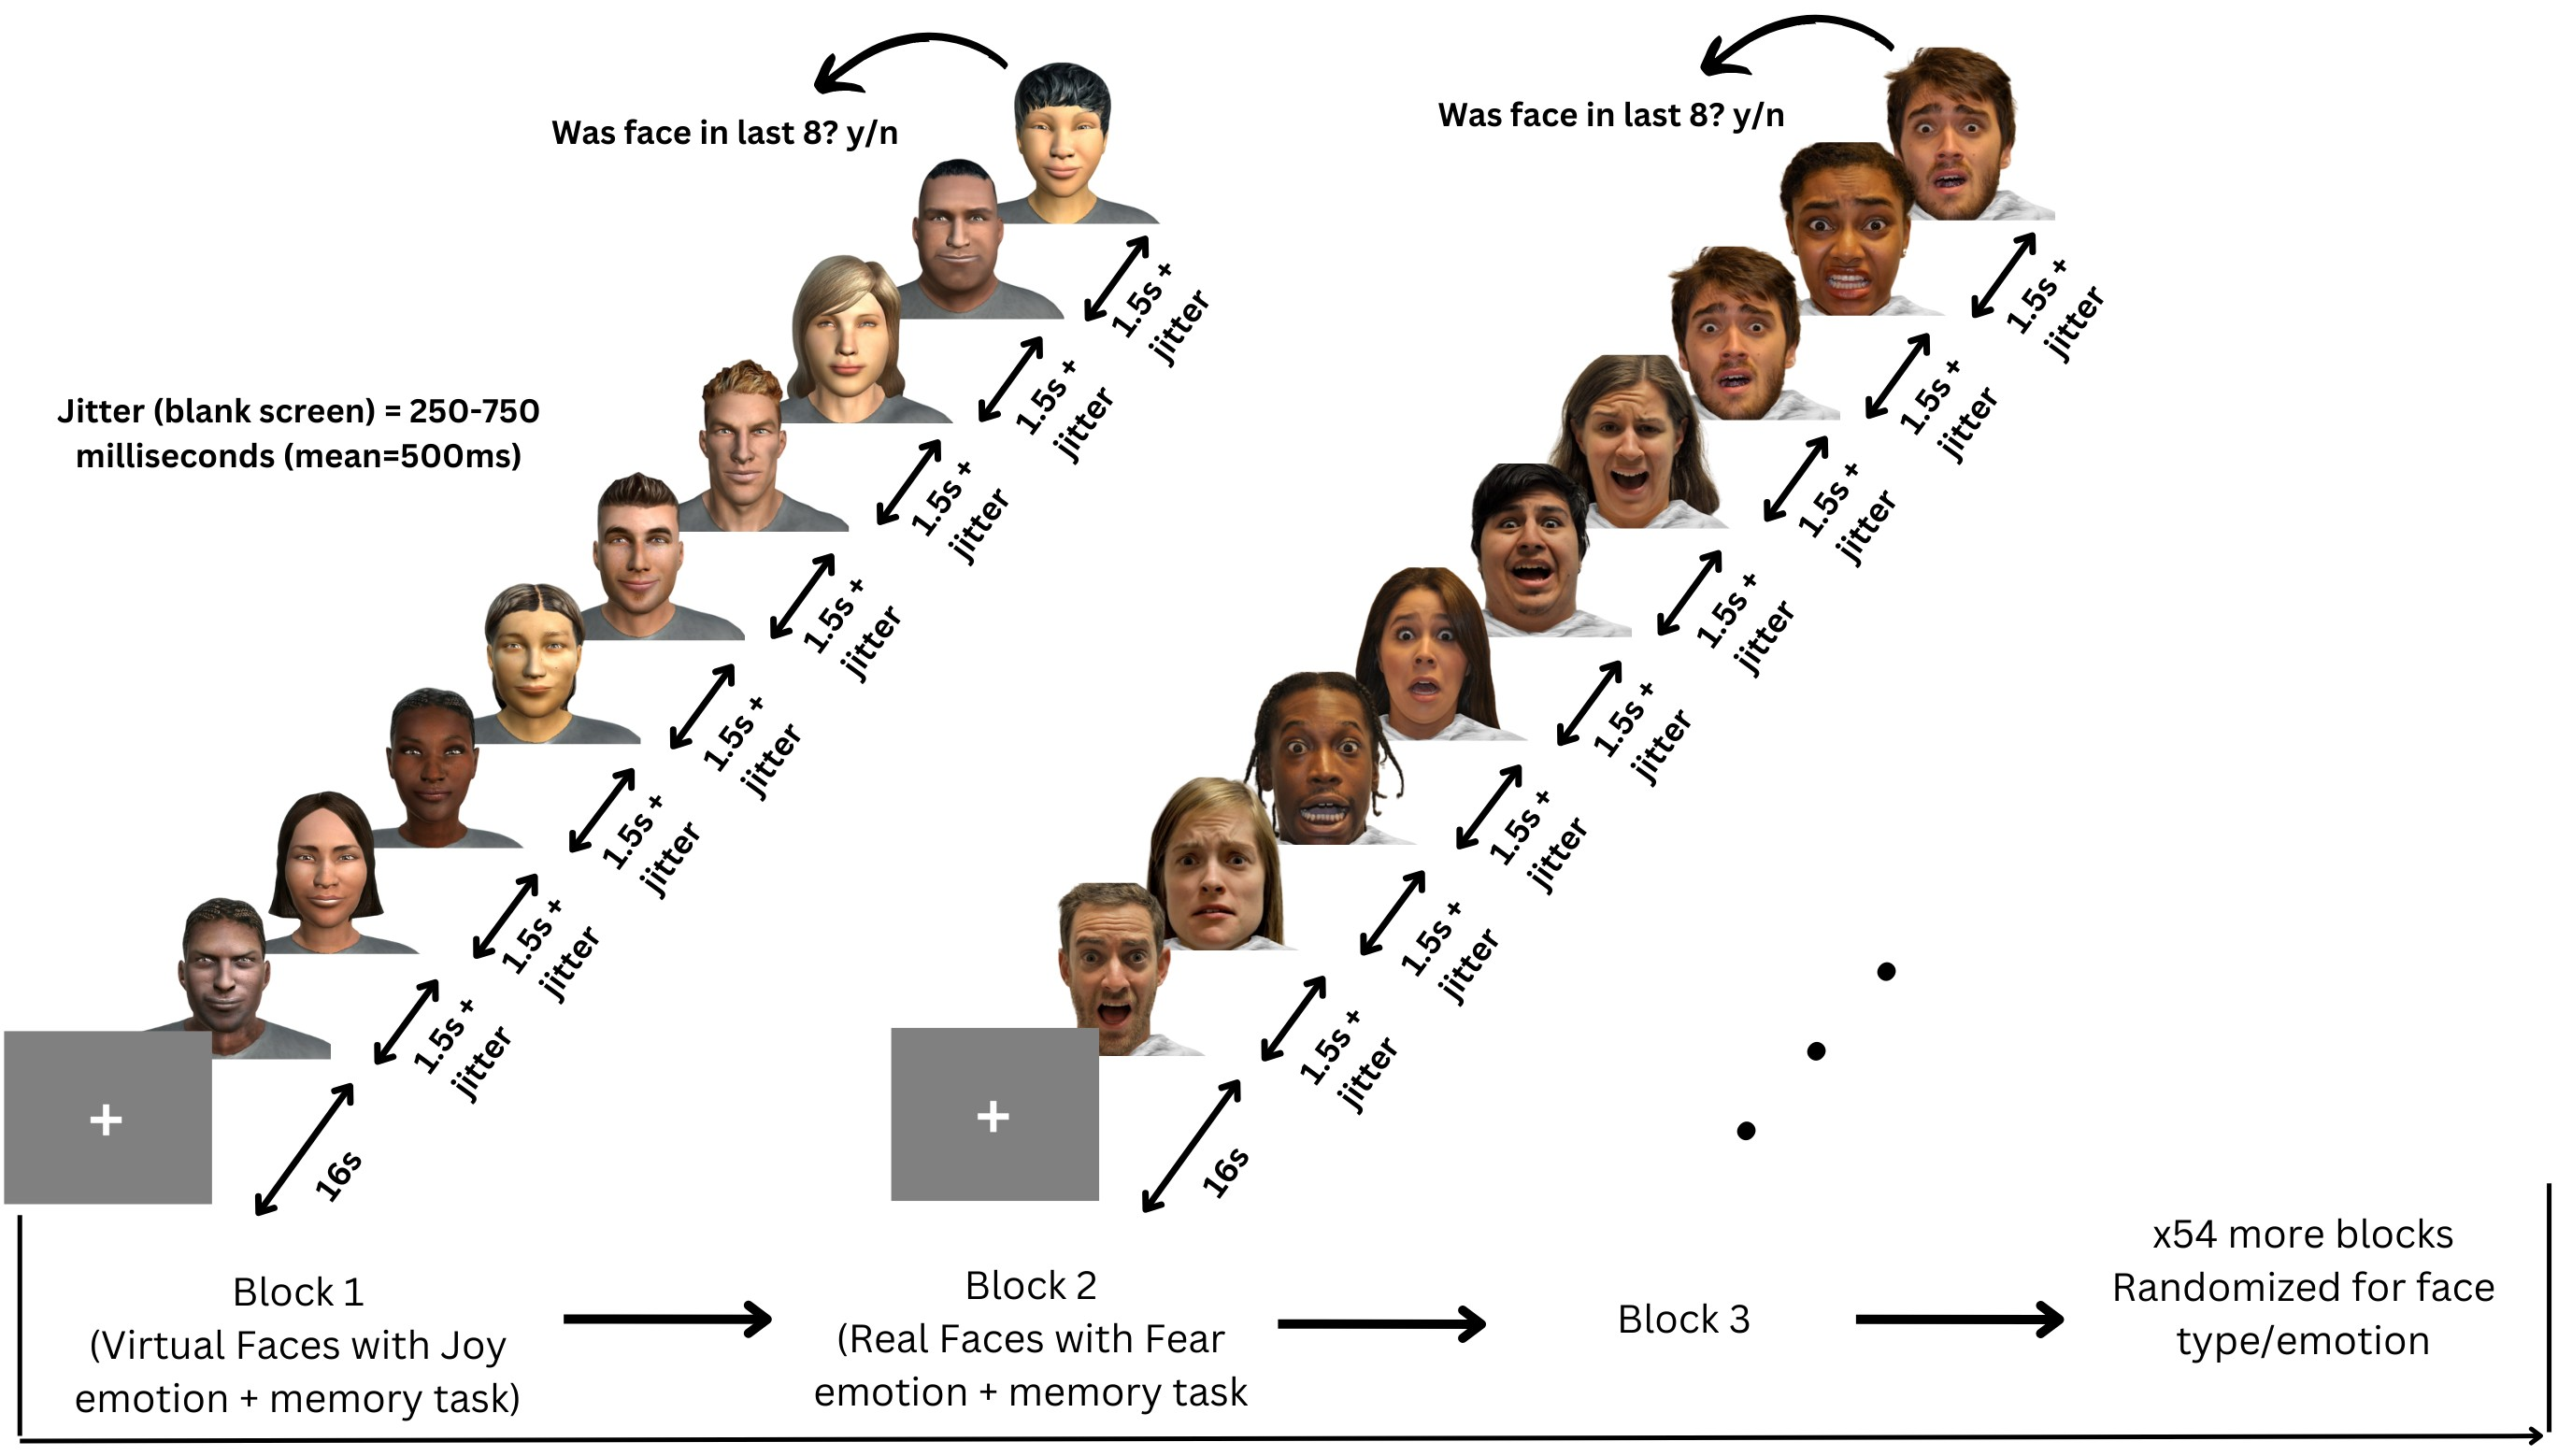
\includegraphics[width=0.9\textwidth]{C:/Users/super/OneDrive - Ontario Tech University/fNIRS_Emotions/plots/figures/Paradigm.jpg}
    \caption{Participants viewed 56 blocks of 8 faces (4 male, 4 female) from two sets:
    real (RADIATE) and virtual (UIBVFED). Each face displayed one of 7 emotions (anger, disgust, fear, happiness, sadness, surprise, neutral). }
    \label{fig:paradigm}
\end{figure}
The stimuli presentation was prepared using PsychoPy3 Experiment Builder (v2024.1.5) \citep{peirce_psychopy2_2019}. 
The stimuli were presented on a Dell U2415 24 inch 1920x1200 60Hz monitor, placed at eye level, and the participants were seated in a comfortable chair facing the monitor.
The beginning of the stimuli presentation had instructions on the screen, which explained the task to the participant, and the participant entered the space bar when they were ready to start the experiment.

The format of the stimuli presentation was as follows: There are 56 blocks in total, each block consists of 8 faces followed by a 9th face.
The faces within each block are either real (from the RADIATE dataset) or virtual (from the UIBVFED dataset), and the faces are presented in a random order.
All faces within a block had one of seven emotional expressions (joy, fear, anger, disgust, sadness, neutral, surprise), and all faces within a block express the same emotion. 
Between every block and starting the experiment, there is a fixation cross presented for 16 seconds. 
The 8 faces (4 male, 4 female, randomly selected) are presented one at a time, for 1.5 seconds each, with a 250-750 ms (mean 500 ms) interstimulus interval (ISI) between each face. 
The 9th face is presented after the 8th face, and the participant must indicate whether the 9th face was in the previous block of 8 faces by pressing 'y' for yes or 'n' for no. 
This task is described in detail in the \textbf{Memory Task} section above. 
The 9th face has a 50\% chance of either being in the previous block or not, and if the participant does not respond within 7 seconds, the presentation will continue to the next block.
Every 7 blocks, the participants are given a break, and prompted to enter the space bar when they are ready to continue the experiment.
The stimuli presentation lasted approximately 35 minutes in total. 
This paradigm is shown in Figure \ref{fig:paradigm}.

\section{Preprocessing Steps}
\begin{figure}[H]
    \centering
    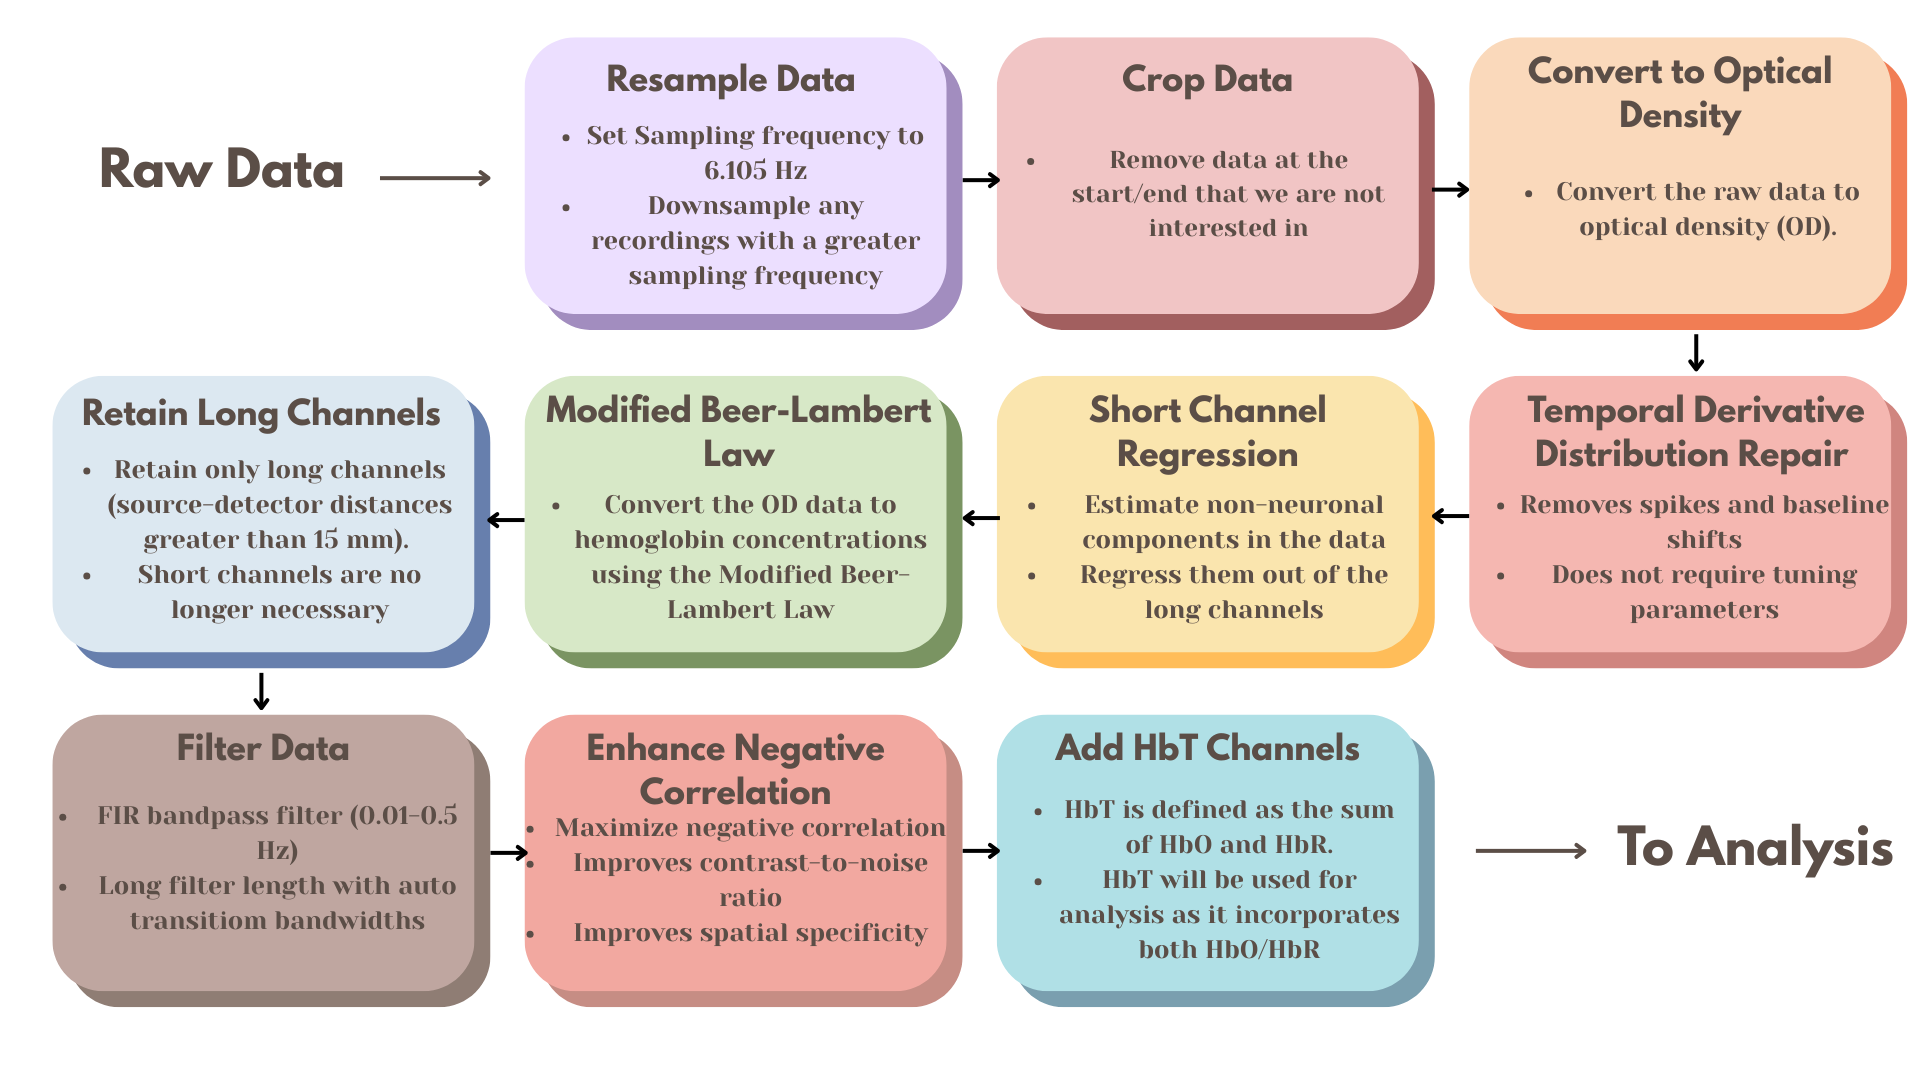
\includegraphics[width=0.9\textwidth]{C:/Users/super/OneDrive - Ontario Tech University/fNIRS_Emotions/plots/figures/Preprocessing Steps.png}
    \caption{Preprocessing steps for fNIRS data, from the raw data to the fully processed data. }
    \label{fig:preprocessing_steps}
\end{figure}

All fNIRS data was preprocessed and analyzed using MNE-Python \citep{gramfort_meg_2013} and MNE-NIRS \citep{luke_analysis_2021}, using Python 3.11.9. 
The preprocessing steps for the fNIRS data (shown in Figure \ref{fig:preprocessing_steps}) were as follows:

\begin{enumerate}
    \item \textbf{Downsample Data:} Downsample the data if the sampling frequency is greater than 6.105 Hz, the initial two datasets were sampled higher than 6.105 Hz, and we want to keep the sampling frequency consistent across all datasets.
    \item \textbf{Crop Data:} Crop the data to the first and last annotation. This gets rid of the extra data at the beginning and end of the recording that we are not interested in.
    \item \textbf{Convert to Optical Density (OD):} Convert the raw data to optical density.
    \item \textbf{Temporal Derivative Distribution Repair (TDDR):} Apply temporal derivative distribution repair to the OD data \citep{fishburn_temporal_2019}. TDDR is effective at removing spikes and baseline shifts from the data. 
    \item \textbf{Short Channel Regression:} Apply short channel regression to the OD data \citep{scholkmann_measuring_2014}. Short channels are used to estimate the superficial hemodynamics (non-evoked/extracerebral/systemic components) in the data, and then regress it out of the long channels \citep{tachtsidis_false_2016}. 
    \item \textbf{Modified Beer-Lambert Law (MBLL):} Convert the OD data to hemoglobin concentrations using the modified Beer-Lambert law. The MBLL relates the change in light attenuation to the change in hemoglobin concentration of chromophores in the tissue \citep{kocsis_modified_2006}.
    \item \textbf{Retain Long Channels:} Retain only long channels (source-detector distance $>$ 15 mm). Since the short channels have already been regressed out, we do not need to keep them in the data.
    \item \textbf{Filter Data:} This FIR bandpass filter extracts signal components in the 0.01-0.5 Hz range, it uses a long filter length (2015 samples) with automatically determined transition bandwidths by MNE-Python \citep{pinti_current_2019}. 
    \item \textbf{Enhance Negative Correlation:} Maximizes negative correlation between HbO and HbR \citep{cui_functional_2010}. This method removes spikes, improves contrast-to-noise ratio, and improves spatial specificity of the data.
    \item \textbf{Add HbT Channels:} Add HbT (hemoglobin total) channels to the data. HbT is defined as the sum of HbO and HbR. Often, fNIRS studies will only use either one of HbO or HbR channels (more frequently HbO), leaving out one channel with no justification \citep{kinder_systematic_2022}. Therefore, we opt to use HbT channels, as technically HbT represents both HbO and HbR channels, and using both hemoglobin species improves the inferences as to where activation occurs \cite{hocke_automated_2018}.
\end{enumerate}
\section{General Linear Model (GLM) Analysis}
\section{Connectivity Analysis}
\section{Building Classifiers}
\section{Memory Task Analysis}